\chapter{RNN ConvNet}
\section*{Local motion}
\begin{figure}[h]
  \centering
  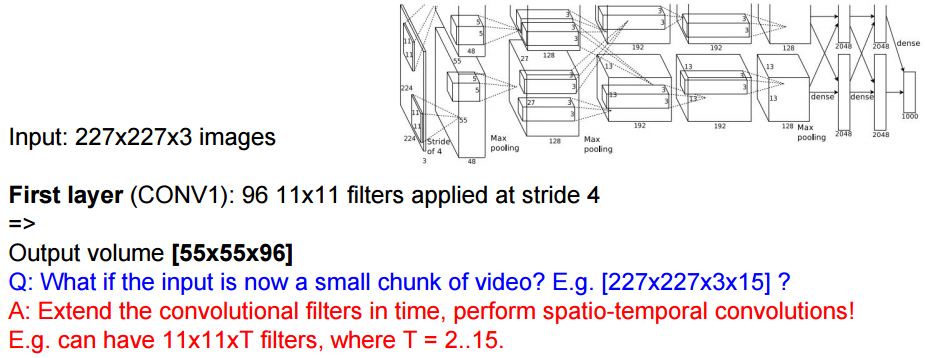
\includegraphics[width=0.6\textwidth]{Images/rnn_convnet/1.png}
  \caption{Getting there}
\end{figure}
\begin{figure}[h]
  \centering
  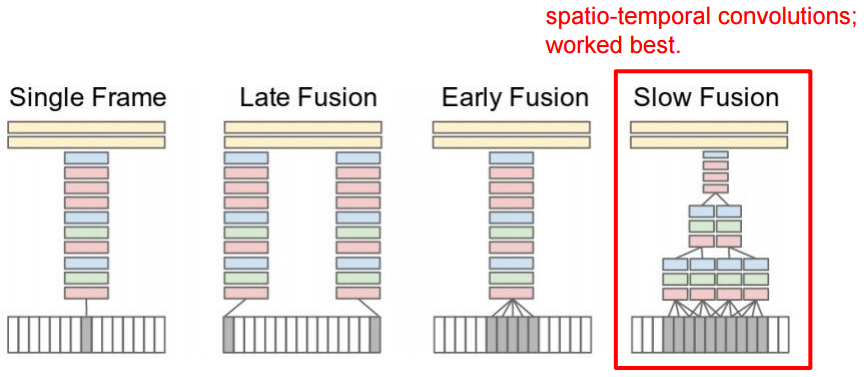
\includegraphics[width=0.5\textwidth]{Images/rnn_convnet/2.png}
  \caption{Large-scale Video Classification with Convolutional Neural Networks, Karpathy et al., 2014]}
\end{figure}

\section*{Global motion}
Delving Deeper into Convolutional Networks for Learning Video Representations, Ballas et al., 2016
\begin{figure}[h]
  \centering
  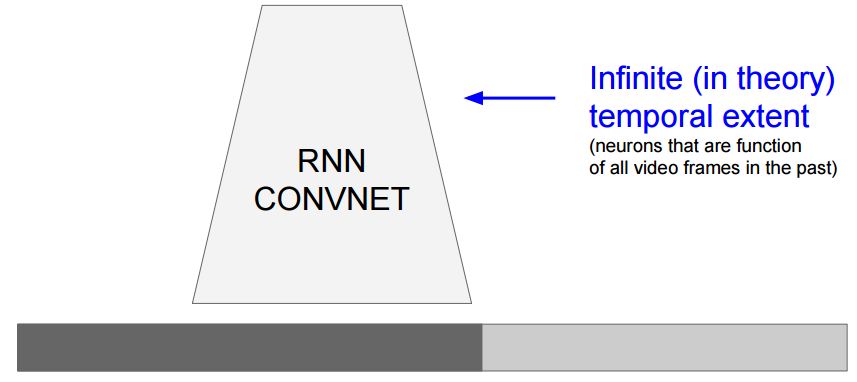
\includegraphics[width=0.35\textwidth]{Images/rnn_convnet/3.png}
  \caption{Large-scale Video Classification with Convolutional Neural Networks, Karpathy et al., 2014]}
\end{figure}
\begin{figure}[h]
  \centering
  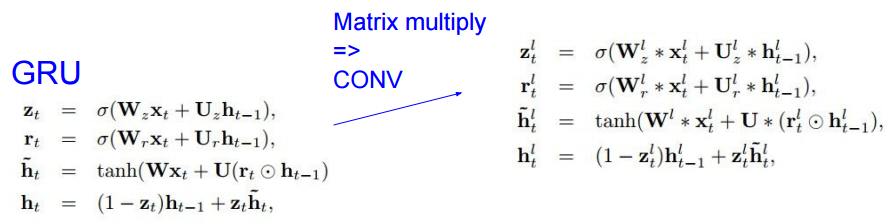
\includegraphics[width=0.75\textwidth]{Images/rnn_convnet/6.png}
  \caption{The idea is to modify GRU adding convolutions. The Gated Recurrent Unit (GRU) is a simplified version of an LSTM unit with fewer parameters. Just like an LSTM cell, it uses a gating mechanism to allow RNNs to efficiently learn long-range dependency by preventing the vanishing gradient problem. The GRU consists of a reset and update gate that determine which part of the old memory to keep vs. update with new values at the current time step.}
\end{figure}
\begin{figure}[h]
  \centering
  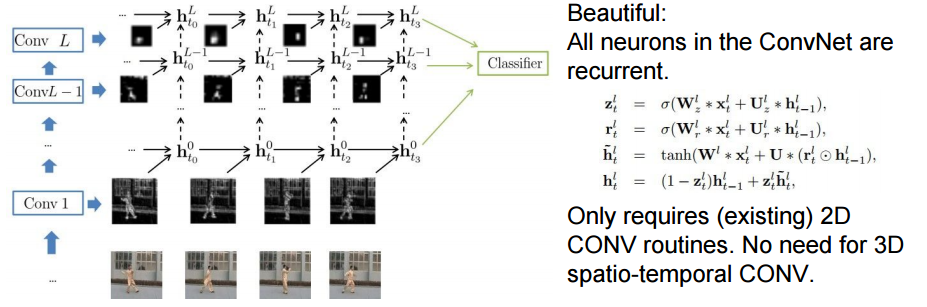
\includegraphics[width=0.65\textwidth]{Images/rnn_convnet/5.png}
  \caption{Original paper diagram}
\end{figure}
\begin{figure}[h]
  \centering
  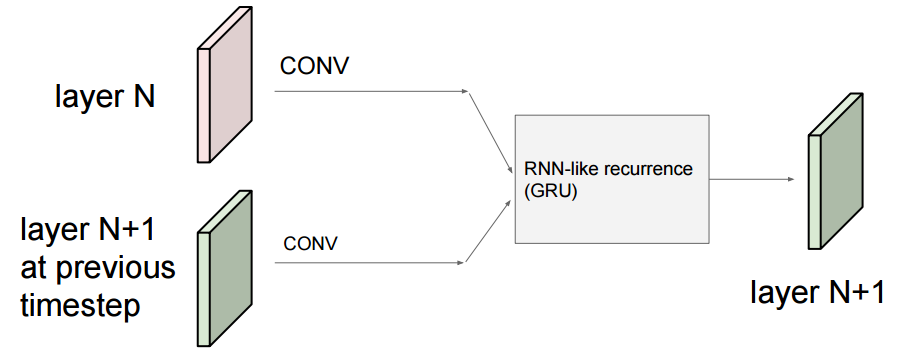
\includegraphics[width=0.45\textwidth]{Images/rnn_convnet/4.png}
  \caption{A more clear diagram}
\end{figure}

\section*{Summary}
\begin{enumerate}
\item You think you need a Spatio-Temporal Fancy VideoConvNet
\item STOP. Do you really?
\item Okay fine: do you want to model:
\begin{itemize}
\item local motion? (use 3D CONV), or
\item global motion? (use LSTM).
\end{itemize}
\item Try out using Optical Flow in a second stream (can workbetter sometimes)
\item Try out GRU-RCN! (imo best model)
\end{enumerate}
